\documentclass[letterpaper, 12pt]{article}

\usepackage[utf8]{inputenc}
\usepackage[english, spanish]{babel}
\usepackage{fullpage}
\usepackage{graphicx}
\usepackage{amsmath}
\usepackage{enumitem}
\usepackage{chngcntr}
\usepackage{setspace}
\usepackage{url}
\usepackage{csquotes}
\usepackage{float}
\usepackage{verbatim}
\usepackage{tabularx}
\usepackage{amsmath}
\usepackage{caption}
\usepackage{bm}
\usepackage{wrapfig}
\usepackage{siunitx}

\counterwithin{figure}{section}
\renewcommand{\thesection}{\arabic{section}}
\renewcommand{\thesubsection}{\thesection.\arabic{subsection}}
\renewcommand{\baselinestretch}{2}
\renewcommand{\thefigure}{\arabic{figure}}

\usepackage[style=numeric, maxnames=6, minnames=3, backend=biber, parentracker=true, sorting=none]{biblatex}
\DefineBibliographyStrings{english}{%chktex-file 1 chktex-file 6
    andothers = {\em et\addabbrvspace al\adddot}
}

\addbibresource{./Bibliography/bibliography.bib}

\usepackage{array}
\usepackage{enumitem}

\setlength{\parskip}{\baselineskip}

\newcommand{\bolditalic}[1]{\textbf{\textit{#1}}}

\DeclareSIUnit{\COP}{COP}
\newcommand{\cop}[1]{\$\SI{#1}{\COP}}

\DeclareSIUnit{\DOLLAR}{USD}
\newcommand{\dollar}[1]{\$\SI{#1}{\DOLLAR}}

% chktex-file 24

\begin{document}

\section*{Análisis: Seguridad en Cartagena de Indias}

\noindent\makebox[\linewidth]{\rule{\textwidth}{0.4pt}}

\begin{itemize}[label=$\diamond$]
    \item Mauro González~\textit{(T00067622)}
    \item Valentina Del Rio~\textit{(T00081360)}
    \item Germán De Armas~\textit{(T00068765)}
\end{itemize}

\noindent\makebox[\linewidth]{\rule{\textwidth}{0.4pt}}

\nocite{fontalvo_leyes2019}

% * REFERENCIAS BY JESS

\nocite{Comunicaciones_2023}
\nocite{Observatorio_2023}
\nocite{MedicinaLegalCienciasForenses_2023}

% * -------------------------------------------------------|>

% ! Introducción

% * Dar una pequeña descripción de la temática
% * ademas de establecer de que se va a hablar
% 

La seguridad en cualquier sociedad es un derecho
fundamental que abarca diversas dimensiones de la vida
cotidiana y que impacta directamente en el bienestar y la
calidad de vida de sus habitantes.

En el contexto de Cartagena de Indias, una ciudad histórica
y turística ubicada en la costa caribeña de Colombia, la
cuestión de la seguridad se presenta como un desafío
multifacético que aborta tanto las dimensiones
tradicionales de la seguridad ciudadana como aquellas que
afectan a los grupos mas vulnerables de la población.

Este trabajo se propone analizar la situación de la
seguridad en Cartagena desde una perspectiva
interdisciplinaria que abarca aspectos cuantitativos y
cualitativos. Se exploraran las políticas publicas de
seguridad ciudadana, condiciones de trabajo en general,
desafíos que enfrenta la ciudad desde hace mas de una
década y seguridad de las mujeres en el contexto urbano. A
través de este análisis, buscamos comprender la complejidad
de la seguridad en Cartagena y contribuir a la discusión de
políticas publicas que promuevan un entorno más seguro y
equitativo para todos los residentes de la ciudad.

% ! ---------------------------------------------------------------------|>

% * --------------------------------------------------------------|>
% * Seguridad Económica 

\subsection*{Seguridad Económica}

Cartagena presenta serios problemas de seguridad desde
tiempo atrás, que hasta la fecha, muchos de estos siguen
sin ser resueltos, o incluso, pueden ser mas graves de lo
que fueron por ejemplo, hace 10 años. La~\textit{Seguridad
    Económica}, es definida como la capacidad de las personas,
los hogares, o las comunidades de satisfacer sus
necesidades básicas de manera sostenible y con
dignidad~\cite{DeLaCruzRoja_2015}. En ese sentido, en
Cartagena se registro un ingreso per cápita durante el año
2020 de tan solo \cop{355004}~\cite{DANE_2021},
representando la linea de pobreza monetaria. Esto se
traduce en \dollar{85} aproximadamente, siendo esto en la
mayoría de casos, mucho menos que suficiente para ``poder
llegar a fin de mes''.

% * --------------------------------------------------------------|>
% * Seguridad Social 

\subsection*{Seguridad Social}

\textsuperscript{1} En una ciudad tan grande y agitada como
lo es Cartagena de Indias, la seguridad ciudadana puede definirse como una
necesidad social. Este concepto se refiere a las exigencias
específicas de la población vinculadas con la delincuencia
y las situaciones de vulnerabilidad y riesgo para sus
personas y bienes, las cuales estarían estrechamente
asociadas a la policía pública, que tiene la función de
resolver, o al menos minimizar, los efectos negativos de
dichas amenazas.

\footnotetext[1]{\cite{fontalvo_leyes2019}. Cita que respalda los
    párrafos siguientes}

En la actualidad la seguridad ciudadana se ve resumida a
soluciones a corto plazo planteadas por los gobiernos
locales que se sienten sectorizadas e insuficientes, para
ser más específicos, los ciudadanos sienten que están
siendo categorizados y excluidos con las políticas
públicas.

Estas políticas implementadas en un territorio determinado
deben tener un papel real en los efectos que desean buscar;
deben verse reflejadas en resultados altamente efectivos de
tal forma que cumplan con el fin último de su acepción como
lo es la garantía y protección de uno o más derechos y la
satisfacción de las necesidades en los habitantes. Sin
embargo, resulta compleja esta garantía si se tiene en
cuenta que las necesidades de los ciudadanos cartageneros
en materia de seguridad se han visto afectadas en gran
manera por factores alternos.

Dentro del marco de lo legal, el desarrollo de las
políticas públicas dentro del plano institucional y su
eficacia social se desarrollan desde tres puntos de
vista~\cite{Thoenig}:

\begin{itemize}
    \item El primero, centrado en el enfoque social, que privilegia
          al individuo y el pluralismo social y solo concibe el
          Estado, desde una perspectiva funcionalista, como una
          ventanilla encargada de atender las demandas sociales.

    \item Un segundo grupo de teorías, al contrario, insiste en
          atribuir al Estado la condición de instrumento al servicio
          de una clase o de grupos específicos. Según esta óptica, el
          Estado dispone sólo de una autonomía marginal, ya
          represente los intereses del capital (teorías neomarxistas)
          o de los burócratas o expertos que lo controlan desde su
          interior (teorías neoweberianas).

    \item Finalmente, un tercer conjunto intenta encontrar un camino
          intermedió, dedicándose a interpretar los equilibrios y
          desequilibrios que se establecen entre el Estado y la
          sociedad y que las políticas públicas permiten traducir.
\end{itemize}

% * --------------------------------------------------------------|>
% * Seguridad Humana

\subsection*{Seguridad Humana}

La seguridad humana es un enfoque crucial que tiene como
objetivo garantizar la supervivencia, los medios de
subsistencia y la dignidad de los ciudadanos en una
sociedad~\cite{DSUAdmin}. Sin embargo, en el contexto de la
ciudad, esta seguridad se ve amenazada por diversas
dificultades que afectan la calidad de vida de sus
habitantes.

Tomando como ejemplo las cifras de delincuencia en la
ciudad~\cite{cifras_crimenes_1}~\cite{cifras_crimenes_2},
las cuales, son un reflejo total de esta problemática. El
miedo a la delincuencia ha llevado a situaciones en las que
muchas personas no se sienten seguras ni siquiera dentro de
sus propias casas.

En este contexto, es imperativo que las políticas públicas
se centren en superar las dificultades generalizadas e
intersectoriales que afectan a la población, con el fin de
garantizar una mayor calidad de vida para sus ciudadanos.
Sin embargo, lamentablemente, la realidad muestra que
muchas personas se ven en la necesidad de velar por su
propia seguridad debido a la poca presencia de los agentes
de control por parte del Estado. Esta situación, a su vez,
genera una brecha de desigualdad, ya que no todos tienen
los medios económicos para darse este ``lujo''.

% ! ---------------------------------------------------------------------|>

% * Insertar here párrafo de transición

% ! ---------------------------------------------------------------------|>

% * --------------------------------------------------------------|>
% * Análisis seguridad en Cartagena

% * --------------------------------------------------------------|>
% * Violencia Intrafamiliar en Cartagena

\subsection*{Violencia intrafamiliar en Cartagena}

\begin{figure}[H]
    \begin{center}
        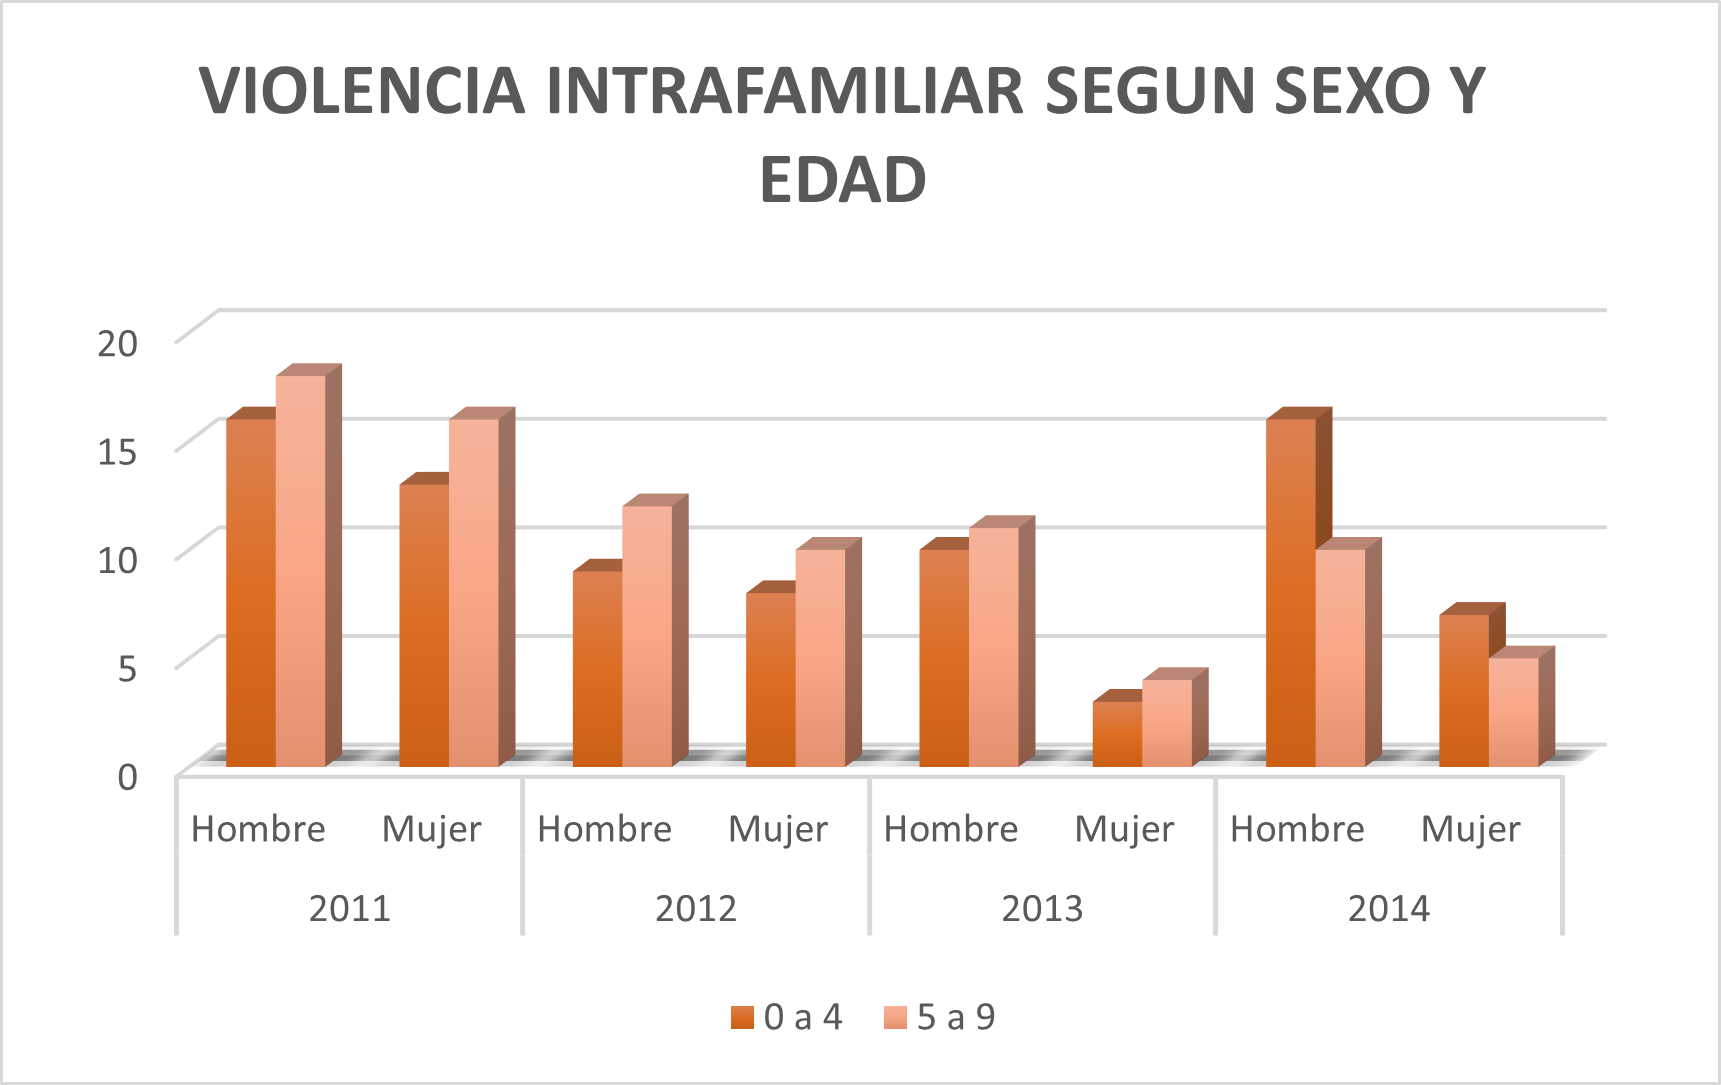
\includegraphics[width=.8\linewidth]{./Images/Graph.ViolenciaIntrafamiliarCartagena.png}
        \caption{Gráfico que muestra la incidencia de violencia intrafamiliar en Cartagena.}
        \label{fig:Graph.ViolenciaIntrafamiliarCartagena}
    \end{center}
\end{figure}

Al analizar la
tabla~\ref{fig:Graph.ViolenciaIntrafamiliarCartagena}, se
destacan varios puntos, siendo uno de ellos la marcada
disparidad de género evidente a lo largo de todos los años
considerados. Se observa que los hombres presentan una
incidencia significativamente superior en comparación con
las mujeres en este aspecto.

Teniendo en cuenta el rango de edad, en 2013, hay una
disminución significativa en la violencia hacia las mujeres
en el rango de 0 a 4 años.

Considerando también los diferentes rangos de edad
afectados en esta problemática,

\begin{itemize}[label=$\diamond$]
    \item En el rango de 0 a 4 años: La tasa de violencia
          intrafamiliar es de $15.67$ por cada 100.000 habitantes.
          Esto significa que, proporcionalmente, 15 niños o niñas son
          víctimas de violencia intrafamiliar por cada 100.000
          habitantes en este grupo de edad.

    \item En el rango de 5 a 9 años: Se observa una leve disminución
          en la tasa de violencia intrafamiliar, la cual se sitúa en
          torno a $13,85$ casos por cada 100.000 habitantes. Esta
          cifra, que representa la incidencia de violencia
          intrafamiliar en la población general, sugiere una
          proporción relativamente baja. En consecuencia, podría
          inferirse que la incidencia de violencia familiar en esta
          área o comunidad específica no es significativamente alta.
\end{itemize}

Es alentador observar una disminución general en los casos
de violencia intrafamiliar a lo largo de estos años. Sin
embargo, la persistencia de casos, especialmente en el
rango de edad de 5 a 9 años, indica que aún hay desafíos
importantes en la prevención de la violencia intrafamiliar,
tales como:

\begin{itemize}[label=$\diamond$]
    \item Subreporte y Estigmatización: Las víctimas, al enfrentar el
          temor a represalias y experimentar vergüenza al momento de
          denunciar, no solo contribuyen a una marcada
          infrarreportación, sino que también alimentan un ciclo de
          repetición constante de la violencia. El miedo a mencionar
          y hablar sobre los incidentes no solo perpetúa el silencio,
          sino que también proporciona un terreno propicio para que
          la violencia persista y se intensifique.

    \item Falta de Conciencia y Educación: La falta de conocimiento
          sobre los signos de violencia intrafamiliar contribuye a
          que los casos pasen desapercibidos, destacando la necesidad
          de sensibilización y educación comunitaria.

    \item Recursos Limitados: La escasez de recursos financieros
          obstaculiza la implementación de programas efectivos,
          incluyendo refugios seguros, servicios de asesoramiento y
          rehabilitación.
\end{itemize}

La diferencia de género es notable, siendo los hombres
quienes experimentan una mayor incidencia en todos los
casos. Esto sugiere la necesidad de programas y políticas
específicas para abordar las causas subyacentes de la
violencia en este contexto.

% * --------------------------------------------------------------|>
% * Muertes violentas en Cartagena

\subsection*{Muertes violentas en Cartagena}

\begin{figure}[H]
    \begin{center}
        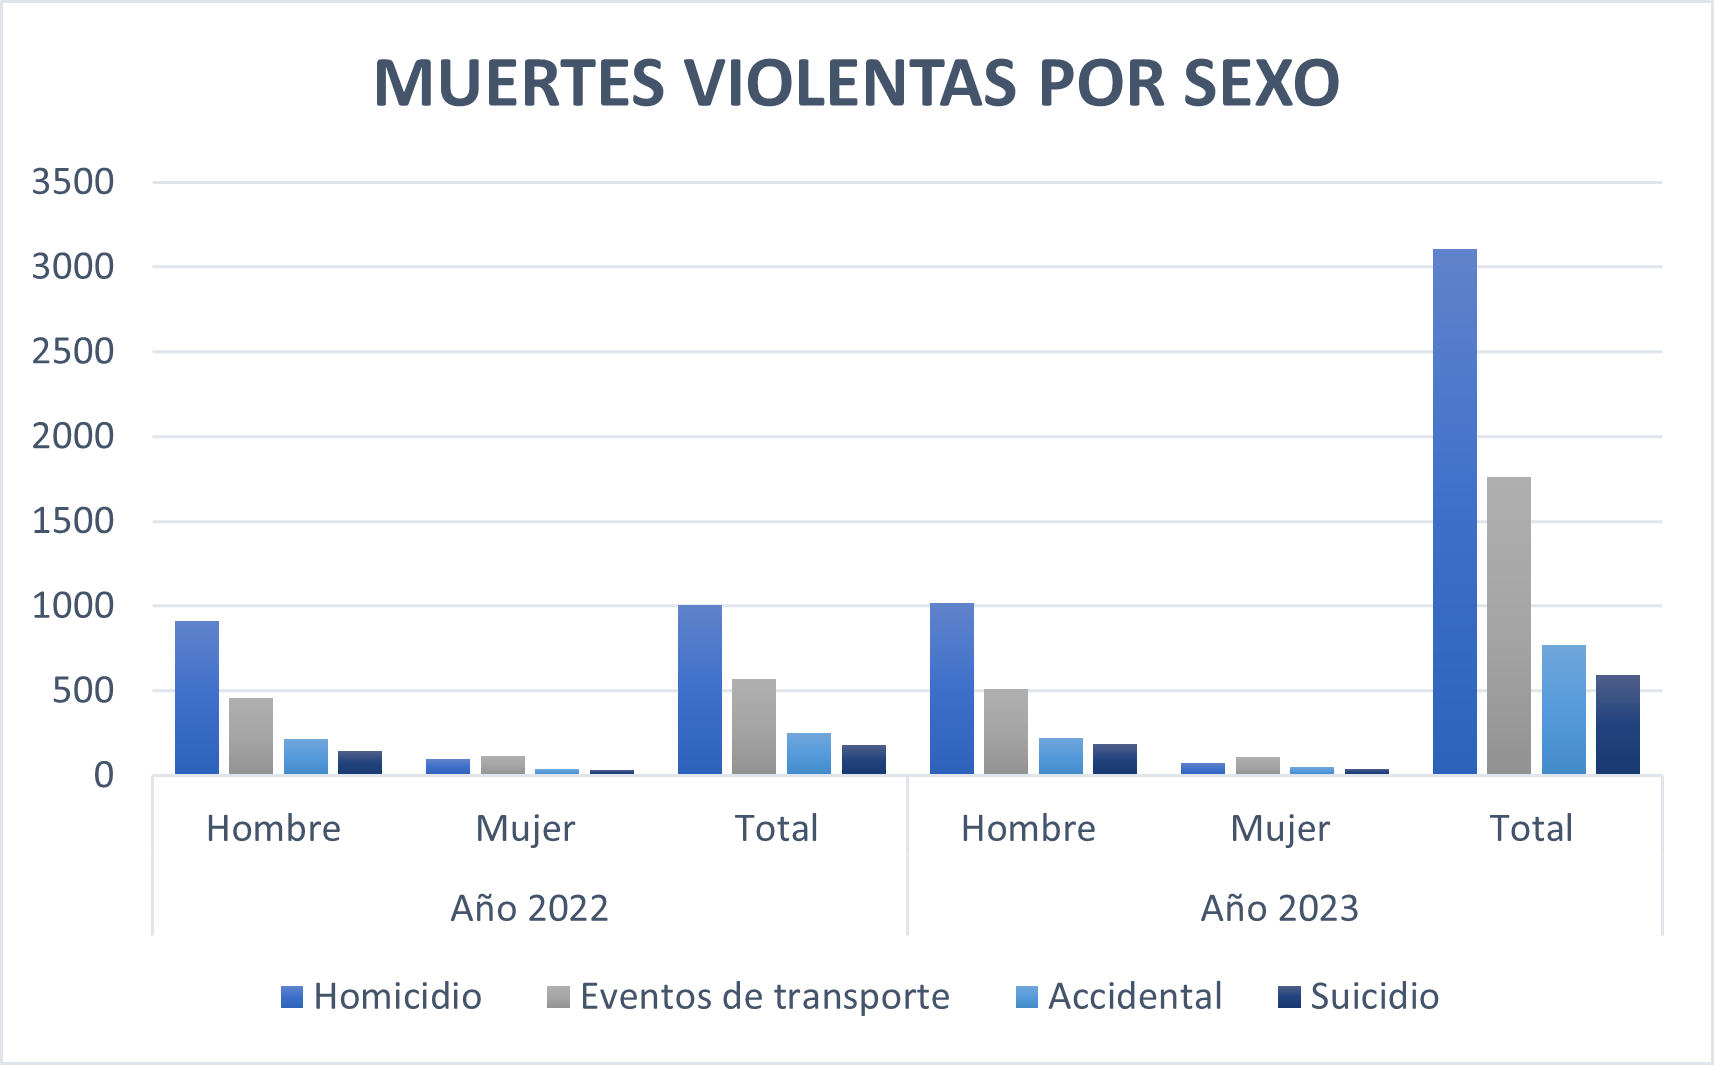
\includegraphics[width=.8\linewidth]{./Images/Graph.MuertesViolentas.png}
        \caption{Gráfico que muestra la cantidad de muertes violentas dependiendo del sexo}
        \label{fig:Graph.MuertesViolentas}
    \end{center}
\end{figure}

Teniendo en cuenta este
aspecto~(\ref{fig:Graph.MuertesViolentas}), hay varios
factores a considerar, como por ejemplo, la gran diferencia
de género que se registró en 2022 con 1.008 homicidios,
registrando de esta manera 911 hombres y 97 mujeres.

En 2023, aunque la cifra total aumentó a 3.106, la
proporción de homicidios entre hombres (1.016) y mujeres
(74) persiste. La alta proporción de homicidios indica la
necesidad de intervenciones específicas para abordar las
causas subyacentes y prevenir la violencia interpersonal.

Basándonos en ello, también es relevante tener en cuenta
los aspectos en los cuales los eventos de transporte
constituyen una causa significativa de muertes violentas.
En 2022, hubo 571 casos, mostrando una diferencia notable
entre hombres (456) y mujeres (115). En 2023, la cifra
total aumentó a 1.763, y la disparidad de género se mantuvo
(513 hombres, 108 mujeres).

La seguridad vial y la educación sobre transporte deben ser
áreas de enfoque para reducir estas muertes, en ese
sentido, se sugiere el desarrollo de campañas de
concientización pública, dirigidas a conductores, peatones
y ciclistas, resaltando la importancia de la seguridad
vial. Además, se intercede por la integración de la
educación vial en el currículo escolar desde temprana edad,
enseñando a los niños sobre normas de tráfico y
comportamientos seguros.

La instauración de programas destinados a promover
prácticas viales seguras y sensibilizar a los conductores
emerge como una medida vital. En pos de mejorar la
infraestructura vial, se sugiere canalizar inversiones
hacia calles más resguardadas, pasos de peatones y carriles
para bicicletas, respaldados por una señalización clara.

La correlación entre las altas cifras de eventos de
transporte y accidentes, que subraya la importancia de
políticas y medidas de seguridad vial, así como el aumento
en los casos de suicidio, destaca la necesidad de abordar
de manera integral la salud pública. Esto implica
incorporar tanto la seguridad en las carreteras como la
promoción activa de la salud mental y la conciencia sobre
el bienestar emocional.

% * --------------------------------------------------------------|>
% * Hurtos en Cartagena

% chktex-file 8
\subsection*{Hurtos en Cartagena 2021-2022}

\begin{figure}[H]
    \begin{center}
        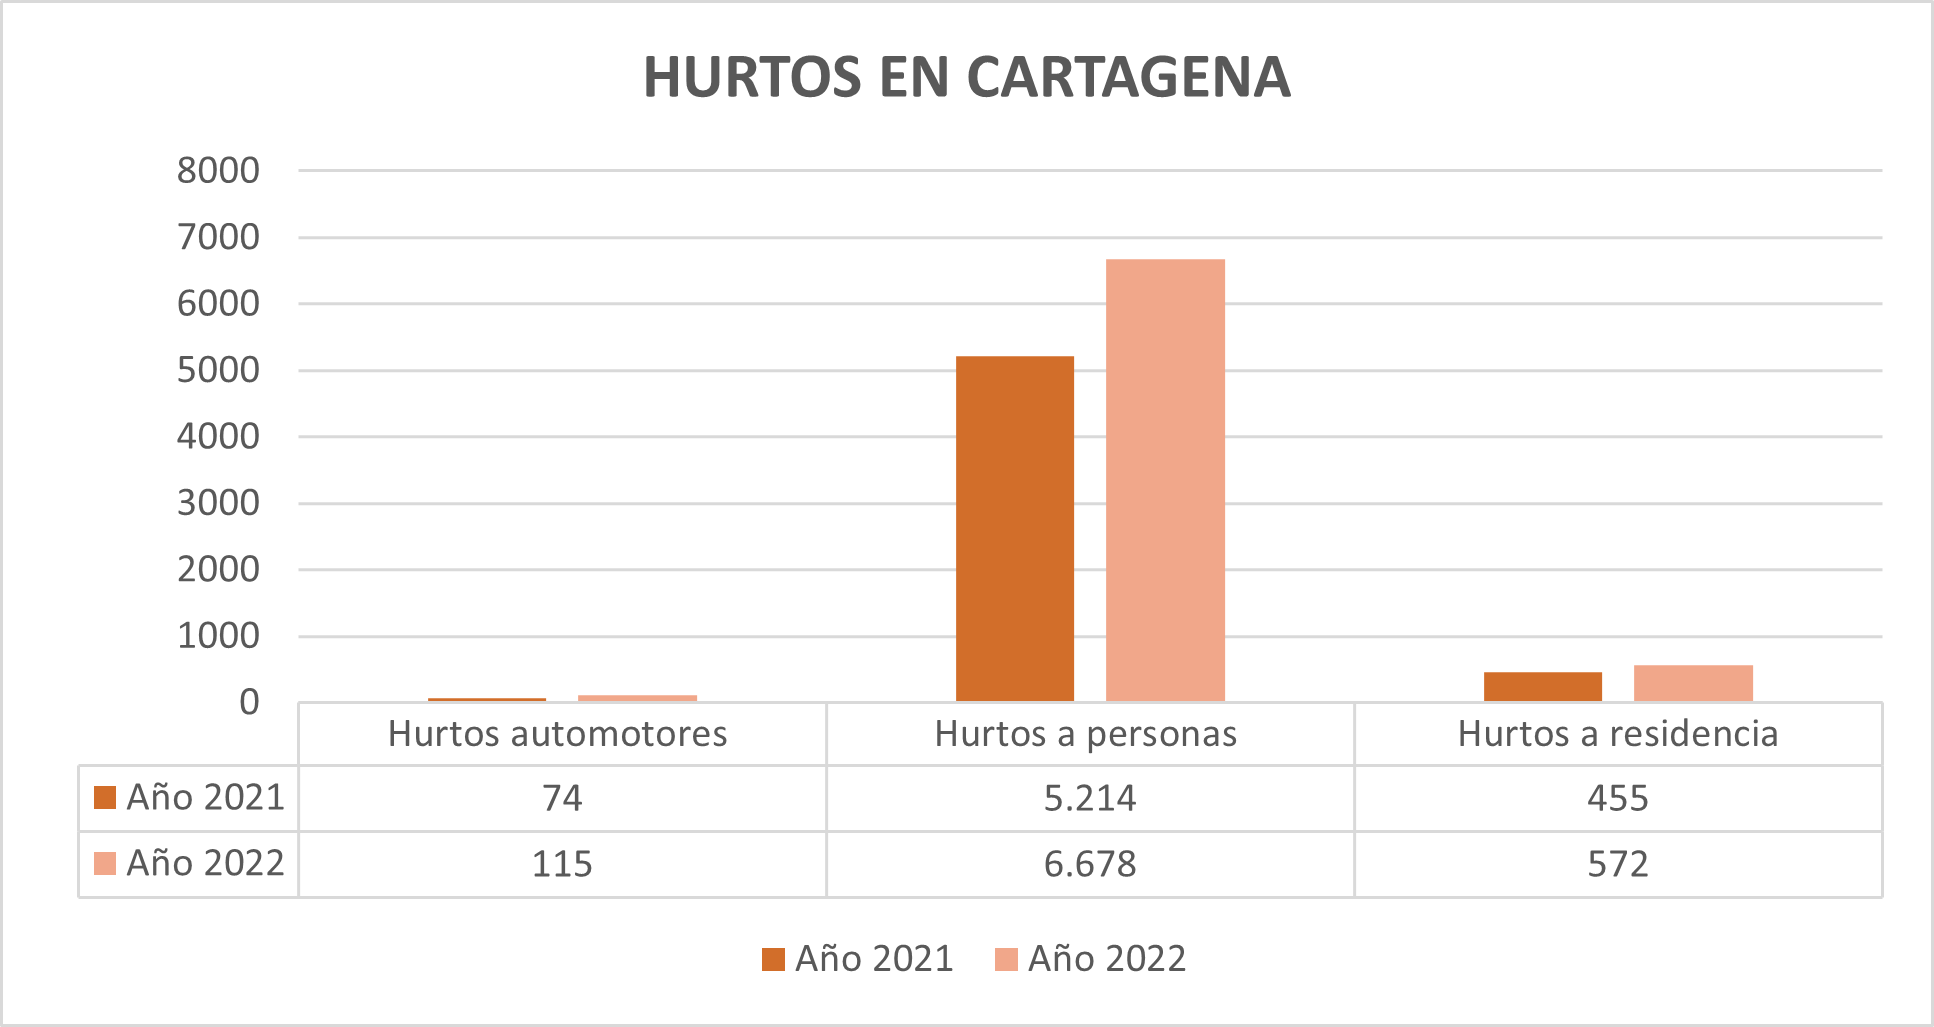
\includegraphics[width=.8\linewidth]{./Images/Graph.HurtosCartagena.png}
        \caption{Hurtos en Cartagena durante el periodo 2021-2022}
        \label{fig:Graph.HurtosCartagena}
    \end{center}
\end{figure}

En este contexto, se destaca que los hurtos de automóviles
experimentaron el mayor incremento, registrando un aumento
del 55.41\% de 2021 a 2022. De manera similar, los robos a
personas se incrementaron en un 28.02\%, y los robos a
residencias subieron un 25.71\% en el mismo período. A
pesar de estos aumentos, la tasa de robos a personas en
Cartagena sigue siendo más baja en comparación con las
cinco principales capitales del país, según los resultados
comparativos.

El incremento en los hurtos a personas y a residencias
indica la importancia de reforzar la seguridad ciudadana y
la vigilancia residencial. Para combatir el aumento de
estos delitos, se deben fortalecer la seguridad en
estacionamientos o implementar tecnologías anti-robos.

Aunque hay un aumento en los índices, Cartagena aún
mantiene una tasa más baja de hurtos a personas en
comparación con otras ciudades, como lo son, Bogotá con la
tasa de hurtos en 1.170, Barranquilla con 1.156 y Medellín
de 1.101, lo que puede sugerir cierto grado de eficacia en
las estrategias de seguridad implementadas hasta ahora o
sencillamente algo de suerte.

% * --------------------------------------------------------------|>
% * Análisis cualitativo

\nocite{necesidades}

Después de meticulosamente explorar la situación de
seguridad en Cartagena, se hace ineludible dirigir nuestra
atención hacia otro aspecto preeminente de la sociedad: su
entramado cultural. En esta urbe, los desafíos en
cuestiones culturales adquieren una relevancia inusitada,
siendo la cultura un factor determinante que permea
diversos aspectos de la vida cotidiana.

Es un axioma reconocido que las acciones humanas están
intrínsecamente vinculadas a las necesidades y desafíos que
impone el entorno circundante. Desde tiempos ancestrales,
las comunidades han surgido como respuesta a la necesidad
primordial de alimentarse y salvaguardar a la familia. Esta
relación intrínseca entre las necesidades humanas y las
decisiones subsiguientes proporciona un trasfondo esencial
para interpretar la actualidad cartagenera.

En este contexto, la realidad observable en Cartagena se
despliega como un cuadro complejo. La ciudad, enfrentando
limitaciones notables en recursos y percepciones
económicas, se ve afectada por condiciones socioeconómicas
que, aunque desafiantes, son intrínsecas a la lucha diaria
de sus habitantes. A pesar de la resiliencia evidente,
estas condiciones contribuyen, de manera insidiosa y
gradual, al incremento de tensiones y conflictos en la
sociedad.

En suma, la interconexión entre las raíces culturales, las
necesidades humanas fundamentales y las condiciones
socioeconómicas complejas destaca la urgencia de abordar
integralmente los desafíos que afectan a Cartagena. Un
análisis más profundo de esta compleja trama revela la
necesidad imperativa de enfoques equitativos y sostenibles
para impulsar el bienestar y la seguridad en esta vibrante
ciudad.

% * --------------------------------------------------------------|>
% * Conclusiones

En conclusión, el análisis exhaustivo de la seguridad en
Cartagena revela una compleja red de desafíos
interrelacionados que abarcan dimensiones económicas,
sociales y culturales. La ciudad enfrenta problemas
significativos en términos de seguridad económica, con
ingresos per cápita que no alcanzan la línea de pobreza,
generando una brecha económica que impacta directamente en
la calidad de vida de sus habitantes.

La seguridad ciudadana y social también emergen como áreas
críticas, con una marcada diferencia de género en casos de
violencia intrafamiliar y homicidios. La falta de eficacia
percibida en las políticas públicas y la necesidad de
abordar las raíces culturales de la violencia subrayan la
complejidad de los desafíos a los que se enfrenta la
ciudad. Además, las tasas de hurtos y robos señalan la
necesidad de estrategias específicas para reforzar la
seguridad ciudadana y residencial.

En este contexto, se destaca la importancia de enfoques
interdisciplinarios que consideren tanto los aspectos
cuantitativos como cualitativos de la seguridad. Para
promover un entorno más seguro y equitativo en Cartagena,
es esencial la implementación de políticas públicas
efectivas, intervenciones económicas y programas educativos
que aborden de manera integral los desafíos identificados.

\printbibliography

\end{document}
